\section{Computational approach}

\subsection{\label{sec:rwa}The rotating-wave approximation}

Models of isolated \qds{} or \qd{} ensembles in which the separation between dots far exceeds a typical interaction length (perhaps through a finite-difference time-domain grid) often use a rotating-wave approximation to great effect in eliminating high-frequency terms in the solution to \cref{eq:liouville} with only a small change in the resulting dynamics.
Assuming the incident radiation takes the form $\vb{E}(t) = \tilde{\vb{E}}(t) \cos(\omega_L t)$
where $\tilde{\vb{E}}(t)$ represents a slowly-varying envelope function, we introduce a unitary transformation $\tilde{\rho} = \hat{U} \hat{\rho} \hat{U}^\dagger$ where $\hat{U} = \mathrm{diag}(1, e^{i \omega_L t})$ to transform \cref{eq:liouville} into a rotating frame,
\begin{equation}
  i \hbar \pdv{\tilde{\rho}}{t} = \commutator{\hat{U} \hat{\mathcal{H}} \hat{U}^\dagger - i \hbar \hat{V}}{\tilde{\rho}} - \hat{\mathcal{D}}\qty[\tilde{\rho}], \quad \hat{V} \equiv \hat{U} \pdv{\hat{U}^\dagger}{t},
  \label{eq:rotating liouville}
\end{equation}
motivating $\hat{U} \hat{\mathcal{H}} \hat{U}^\dagger - i \hbar \hat{V} \equiv \tilde{\mathcal{H}}$ as a ``rotating-frame Hamiltonian.''
By neglecting the $e^{i \qty(\omega_0 + \omega_L) t}$ terms under the assumption that they oscillate quickly and will therefore integrate to zero over any appreciable timescales, we produce a governing equation much more amenable to numerical integration as it contains only smooth (low-frequency) quantities.

A similar transformation applies to the source distribution in \cref{eq:total field}.
Writing $\vb{P}(\vb{r}, t) = \tilde{\vb{P}}(\vb{r}, t)e^{i \omega_L t}$, the radiated field envelope becomes
\begin{widetext}
\begin{equation}
  \begin{gathered}
    \tilde{\vb{E}}_\text{rad}(\vb{r}, t) = -\frac{1}{4\pi \varepsilon} \int 
    \qty(\tensor{\mathrm{I}} -  \hat{\vb{r}}\hat{\vb{r}}) \cdot \frac{\qty(\partial_t^2 \tilde{\vb{P}}(\vb{r}', t_R) + 2 i \omega_L \partial_t \tilde{\vb{P}}(\vb{r}', t_R) - \omega_L^2 \tilde{\vb{P}}(\vb{r}', t_R)) e^{-i \omega_L \abs{\vb{r} - \vb{r}'}/c}}{c^2 \abs{\vb{r}-\vb{r}'}} + \\
    \qty(\tensor{\mathrm{I}} - 3\hat{\vb{r}}\hat{\vb{r}}) \cdot \frac{\qty(\partial_t \tilde{\vb{P}}(\vb{r}', t_R) + i \omega_L \tilde{\vb{P}}(\vb{r}', t_R))e^{-i \omega_L \abs{\vb{r} - \vb{r}'}/c}}{c \abs{\vb{r}-\vb{r}'}^2} +
    \qty(\tensor{\mathrm{I}} - 3\hat{\vb{r}}\hat{\vb{r}}) \cdot \frac{                \tilde{\vb{P}}(\vb{r}', t_R) e^{-i \omega_L \abs{\vb{r} - \vb{r}'}/c}}{\abs{\vb{r}-\vb{r}'}^3}
    \, \dd[3]{\vb{r'}}.
  \end{gathered}
  \label{eq:radiated envelope}
\end{equation}
\end{widetext}
Critically, \cref{eq:radiated envelope} maintains the phase relationship between every pair of \qds{} for arbitrarily large timesteps via the $e^{-i \omega_L \abs{\vb{r} - \vb{r}'}/c}$ factors that appear.
Without this transformation, the evolution of \cref{eq:liouville} would require $c \, \Delta t$ at least as small as the minimum separation between \qds{}---roughly three orders of magnitude smaller than the $\Delta t$ required to resolve the maximum frequency in \cref{eq:rotating liouville}.

\subsection{Solution of the Liouville equation}

Solving \cref{eq:liouville} for each of $n_s$ \qds{} amounts to solving $n_s$ implicitly coupled first-order differential equations in time.
Due to its extreme accuracy and inherent bandlimitedness, we instead make use of the highly-tuned predictor/corrector scheme detailed in~\cite{Glaser2009} to numerically solve \cref{eq:liouville} for each \qd{} in the system.
Approximating $\hat{\rho}_i(t)$ as a weighted sum of complex exponentials, the predictor/corrector scheme proceeds with an extrapolation predictor step,
\begin{equation}
  \hat{\rho}_i(t_{k + 1}) \coloneqq \sum_{\ell = 1}^k \mathcal{P}_\ell^{\qty(0)} \hat{\rho}_i(t_\ell) + \mathcal{P}_\ell^{\qty(1)} \dot{\hat{\rho}}_i(t_\ell),
  \label{eq:predictor}
\end{equation}
and several iterated corrector steps,
\begin{equation}
  \hat{\rho}_i(t_{k + 1}) \coloneqq \mathcal{C}_{k+1}^{\qty(1)} \dot{\hat{\rho}}_i(t_{k + 1}) + \sum_{\ell = 1}^k \mathcal{C}_\ell^{\qty(0)} \hat{\rho}_i(t_i) + \mathcal{C}_\ell^{\qty(1)} \dot{\hat{\rho}}_i(t_\ell).
  \label{eq:corrector}
\end{equation}
where the $\mathcal{P}_\ell^{\qty(0, 1)}$ and $\mathcal{C}_\ell^{\qty(0, 1)}$ coefficients arise from a least-squares solution to a system of complex-valued exponentials on a semidisk in the left complex plane.

The approximation used in \cref{eq:rotating liouville} facilitates large timesteps that encompass many \qds{}.
These dots interact continuously over each timestep, thus a suitable integrator should accommodate multiple scattering events occurring within the same time interval---a feat accomplished naturally through iterated applications of \cref{eq:corrector}.
Moreover, the coupling term in \cref{eq:hamiltonian} and the retardation factor in \cref{eq:total field} add significant complexities, making ``straightforward'' solution methods (such as RK4 or other midstep methods) ill-suited for the problem at hand.
The necessity of a midstep RHS evaluation in RK4 schemes, for instance, proves troublesome; as the RHS to evaluate a given $\dot{\hat{\rho}}_i$ between timesteps depends on every other $\hat{\rho}_j$ at the same timepoint, the system requires either an infinite number of step subdivisions or some sort of extrapolation scheme to advance by $\Delta t$.
As the predictor/corrector method presented here possesses superior accuracy properties alongside a rigorous extrapolation scheme (by construction), it very naturally solves the system described by \cref{eq:rotating liouville,eq:radiated envelope}.

\subsection{Evaluation of radiated fields}

To evaluate \cref{eq:radiated envelope} between every pair of points we make use of variable-order Lagrange interpolation.
Such a scheme easily accommodates both retardation effects between \qds{} separated by a non-integer number of timesteps as well as the first and second time derivatives of $\vb{P}$.
To make the interpolation calculation as efficient as possible at each timestep, we store only $\qty{f, \vb{c}}$ for every pair of \qds{} where
$f \equiv \lfloor \abs{\Delta \vb{r}}/(c \, \Delta t) \rfloor$ and gives the start of the ``interpolation window'' of width $w$ (\cref{fig:interpolation}) and 
\begin{widetext}
\begin{equation}
  \qty(\vb{c})_n = -\frac{\vb{d}_j}{4\pi \epsilon} \cdot \qty[\qty(I - 3\bar{\vb{r}}\bar{\vb{r}}) \qty(\frac{\ell_n(s)}{\abs{\vb{r}_j - \vb{r}_i}^3} + \frac{\dot{\ell}_n(s) + i \omega_L \ell_n(s)}{c \abs{\vb{r}_j - \vb{r}_i}^2}) +
    \qty(I - \bar{\vb{r}}\bar{\vb{r}}) \frac{\ddot{\ell}_n(s) + 2i \omega_L \dot{\ell}_n(s) - \omega_L^2 \ell_n(s)}{c^2 \abs{\vb{r}_j - \vb{r}_i}}] \cdot \vb{d}_i e^{-i \omega_L \abs{\vb{r}_j - \vb{r}_i}/c}
    \label{eq:interpolation coefs}
\end{equation}
\end{widetext}
where
\begin{align}
  s         &\equiv \abs{\Delta \vb{r}}/\qty(c \, \Delta t) - \lfloor \abs{\Delta \vb{r}}/\qty(c \, \Delta t) \rfloor \label{eq:fractional part} \\
  \ell_n(t) &\equiv \prod_{j = 0}^{-w} \frac{t - j}{n - j}; \quad j \not = n. \label{eq:lagrange polynomial}
\end{align}
Note that the product in \cref{eq:lagrange polynomial} runs over a negative window due to the backwards-looking interpolation.

\begin{figure}
  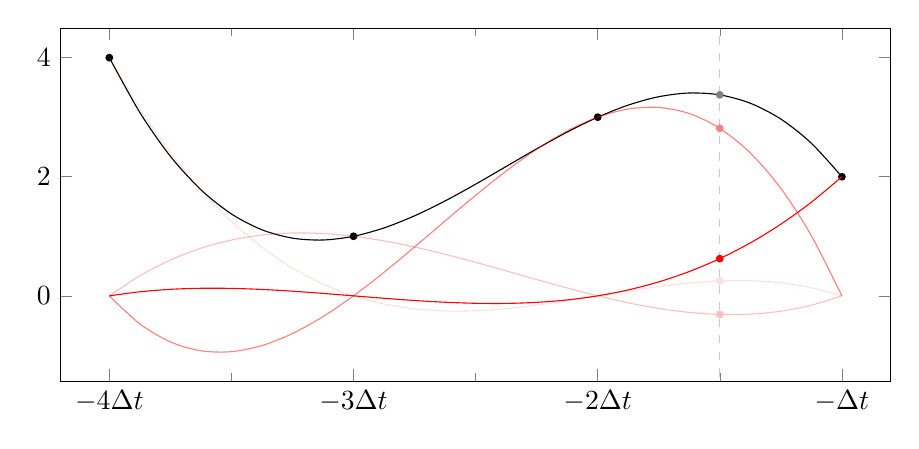
\begin{tikzpicture}
  \begin{axis}[xmin=-4.2, xmax=-0.8, width=\columnwidth, height=0.5\columnwidth,
      xtick={-4, -3, -2, -1},
      minor x tick num={1},
      xticklabels={$-4\Delta t$, $-3\Delta t$, $-2\Delta t$, $-\Delta t$}
  ]

  \addplot[smooth,domain=-4:-1]{2/3*(-3-x)*(-2-x)*(-1-x) + 1/2*(-2-x)*(-1-x)*(4+x) + 3/2*(-1-x)*(3+x)*(4+x) + 1/3*(2+x)*(3+x)*(4+x)};
  \node [fill, black, circle, inner sep=1.0pt] (x1) at (axis cs:-1,2) {};
  \node [fill, black, circle, inner sep=1.0pt] (x2) at (axis cs:-2,3) {};
  \node [fill, black, circle, inner sep=1.0pt] (x2) at (axis cs:-3,1) {};
  \node [fill, black, circle, inner sep=1.0pt] (x2) at (axis cs:-4,4) {};

% Unweighted basis polynomials
  %\draw[dashed, opacity=0.2] (axis cs:-1.2,-10) -- (axis cs:-1.2,10) {};
  %\node [fill, gray, opacity=1.00, circle, inner sep=1.0pt] (pol) at (axis cs:-1.2,2.824) {};

  %\addplot[red, opacity=1.00, smooth, domain=-4:-1]{1/6*(2+x)*(3+x)*(4+x)};
  %\addplot[red, opacity=0.50, smooth, domain=-4:-1]{1/2*(-1-x)*(3+x)*(4+x)};
  %\addplot[red, opacity=0.25, smooth, domain=-4:-1]{1/2*(-2-x)*(-1-x)*(4+x)};
  %\addplot[red, opacity=0.12, smooth, domain=-4:-1]{1/6*(-3-x)*(-2-x)*(-1-x)};

  %\node[fill, red,            circle, inner sep=1.0pt] (p1) at (axis cs:-1.2,0.672) {};
  %\node[fill, red!50!white,   circle, inner sep=1.0pt] (p2) at (axis cs:-1.2,0.504) {};
  %\node[fill, red!25!white,   circle, inner sep=1.0pt] (p3) at (axis cs:-1.2,-0.224) {};
  %\node[fill, red!12.5!white, circle, inner sep=1.0pt] (p4) at (axis cs:-1.2,0.048) {};

% Weighted basis polynomials
  \draw[dashed, opacity=0.2] (axis cs:-1.5,-10) -- (axis cs:-1.5,10) {};
  \node [fill, gray, opacity=1.00, circle, inner sep=1.0pt] (pol) at (axis cs:-1.5,3.375) {};

  \addplot[red, opacity=1.00, smooth, domain=-4:-1]{1/3*(2+x)*(3+x)*(4+x)};
  \addplot[red, opacity=0.50, smooth, domain=-4:-1]{3/2*(-1-x)*(3+x)*(4+ x)};
  \addplot[red, opacity=0.25, smooth, domain=-4:-1]{1/2*(-2-x)*(-1-x)*(4+x)};
  \addplot[red, opacity=0.12, smooth, domain=-4:-1]{2/3*(-3-x)*(-2-x)*(-1-x)};

  \node[fill, red,            circle, inner sep=1.0pt] (p1) at (axis cs:-1.5,0.625) {};
  \node[fill, red!50!white,   circle, inner sep=1.0pt] (p2) at (axis cs:-1.5,2.8125) {};
  \node[fill, red!25!white,   circle, inner sep=1.0pt] (p3) at (axis cs:-1.5,-0.3125) {};
  \node[fill, red!12.5!white, circle, inner sep=1.0pt] (p4) at (axis cs:-1.5,0.25) {};

  \end{axis}
\end{tikzpicture}

  \caption{\label{fig:interpolation}Illustration of interpolation for a $w = 4$ window.
    An assumed signal takes $1.5\Delta t$ to travel from point A to B (dashed line).
    To calculate the electric field at A in the present, we interpolate known values of a source quantity at B (black dots) about the fractional timestep with a sum of weighted basis polynomials (red lines, \cref{eq:lagrange polynomial}) evaluated at the fraction.
  }
\end{figure}
